\documentclass{beamer}

\usepackage[latin1]{inputenc}
\usepackage{algorithmic}
\usepackage{amsmath}
\usepackage{graphicx}
\usepackage{verbatim}
\usepackage{hyperref}

\title{Super-Resolution From a Single Image}
\author{Geoffrey Ulman}
\date{April 21, 2012}
\begin{document}

%%%%%%%%%%%%%%%%%%%%%%%%%%%%%%%%%%%%%%%%%%%%%%%%%%%%

\begin{frame}
\titlepage
\end{frame}

%%%%%%%%%%%%%%%%%%%%%%%%%%%%%%%%%%%%%%%%%%%%%%%%%%%%

\begin{frame}{Original Paper}

Super-Resolution From a Single Image

\vspace{1cm}

\emph{Daniel Glasner, Shai Bagon, Michal Irani}

\vspace{1cm}

\url{http://www.wisdom.weizmann.ac.il/~vision/SingleImageSR.html}

\end{frame}

%%%%%%%%%%%%%%%%%%%%%%%%%%%%%%%%%%%%%%%%%%%%%%%%%%%%

\begin{frame}{Multiple Frame Super-Resolution}

\begin{figure}
\centering
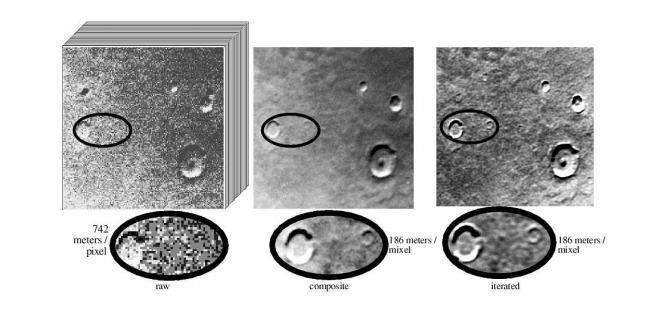
\includegraphics[width=1.0\textwidth]{presentation_screen1.png}
\caption{Multiple images of the same scene with sub-pixel shifts\footnote[1]{\url{http://www.robots.ox.ac.uk/~elle/pubs/elle-thesis.pdf}}}
\end{figure}

\end{frame}


%%%%%%%%%%%%%%%%%%%%%%%%%%%%%%%%%%%%%%%%%%%%%%%%%%%%

\begin{frame}{Multiple Frame Super-Resolution}

Let \( {L_1,...,L_n} \) be a set of images of the same scene.

\vspace{0.3cm}

Assume these images were all derived from a high resolution source image \(H\).

\vspace{0.3cm}

Each low resolution image \(L_j\) was generated by \emph{blurring} and \emph{subsampling} from \(H\).

\vspace{0.3cm}

The \emph{blurring} operation is a convolution with a Gaussian (or similar) kernel \(B_j\).

\begin{figure}
\begin{equation}
\begin{aligned}
L_j = \left( H \otimes B_j \right) \left( q \right) \downarrow s_j
\end{aligned}
\end{equation}
\end{figure}

\end{frame}

%%%%%%%%%%%%%%%%%%%%%%%%%%%%%%%%%%%%%%%%%%%%%%%%%%%%

\begin{frame}{Multiple Frame Super-Resolution}

We can write an equation describing each pixel \(L_j(p)\) of the low resolution image in terms of nearby pixels \(H(q_i)\) in the high resolution image.

\begin{figure}
\begin{equation}
\begin{aligned}
L_j(p) = \sum_{q_i \in Support(B_j)} H( q_i ) B_j( q_i - q )
\end{aligned}
\end{equation}
\end{figure}

For large enough \(j\) this system becomes \emph{over determined} and we can use least squares to approximate the unknown pixels \(H(q)\) in the high resolution image.

\end{frame}

%%%%%%%%%%%%%%%%%%%%%%%%%%%%%%%%%%%%%%%%%%%%%%%%%%%%


\end{document}
